\section{FOUR-SHIP TACTICS}

\subsection{OFFENSIVE TACTICS}

\begin{tcoloritemize}
    \blueitem[Wall]
    Flight goes line abreast
    \hfill\textbf{see \cref{fig:ttp_aa:4ship:offensive:wall}}
    \begin{itemize}
        \item \textbf{maximizes weapon employment capability}
        \item maximizes sensor coverage \& overlap
    \end{itemize}
    
    \blueitem[Use Cases]
    \begin{itemize}
        \item Sweep --- clear airspace of threats
        \item Escort --- sanitize airspace in front of friendlies
    \end{itemize}
\end{tcoloritemize}

\begin{figure}[htbp]
    \centering
    \begin{tikzpicture}[figstyle]

        % coordinates
        \coordinate (lead_lead) at (0,0);
        \coordinate (lead_wing) at (-15,0);
        \coordinate (elem_lead) at (15,0);
        \coordinate (elem_wing) at (30,0);
        \coordinate (bandit) at (7.5,40);
        \coordinate (bandit_wing) at (2.5,45);

        % fighter wez
        \draw[fill=color2!15] 
            \foreach \n in {lead_lead, lead_wing, elem_lead, elem_wing} {
                (\n) -- ++(60:25) arc (60:120:25) -- cycle
            };

        % fighters
        \foreach \n in {lead_lead, lead_wing, elem_lead, elem_wing} {
            \node[] (\n_fig) at (\n) {
                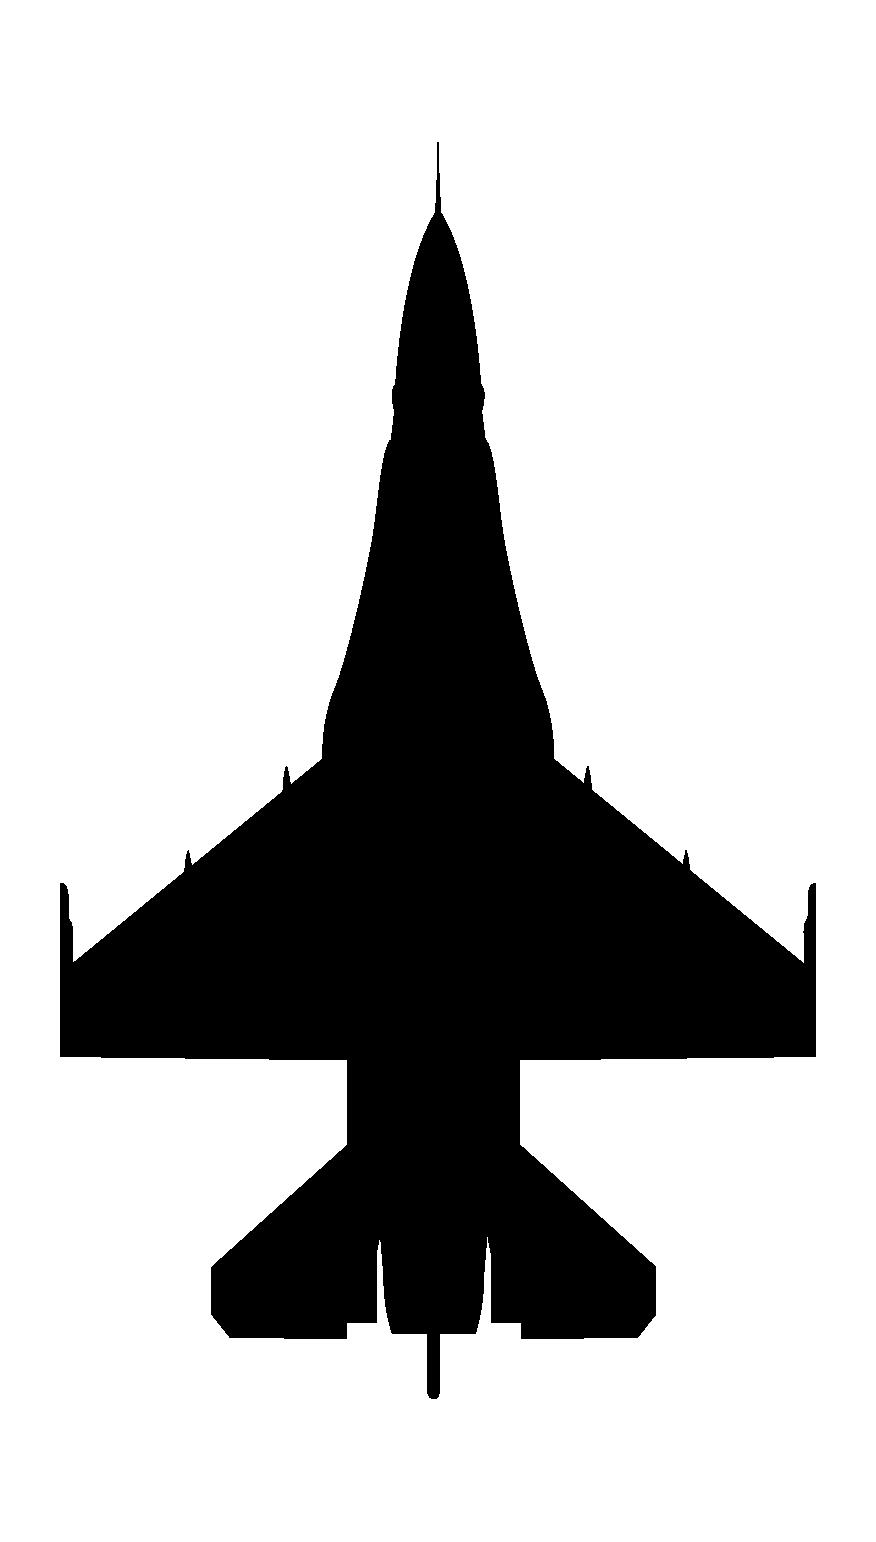
\includegraphics[
                    width=7.5mm,
                ]{diagrams/aircraft/silhouette_f16_top.pdf}
            };
        }

    \end{tikzpicture}
    \caption{Four-ship wall tactics}%
    \label{fig:ttp_aa:4ship:offensive:wall}
\end{figure}

\notebox{
    \small Wall tactics are \textbf{NOT} limited to four-ship, 
    8-ship wall also typical, depends on threat environment.
}

\clearpage

\begin{tcoloritemize}
    \blueitem[Grinder]
    Flight splits into elements, enter racetrack pattern\\
    \hfill\textbf{see \cref{fig:ttp_aa:4ship:offensive:grinder}}
    \begin{itemize}
        \item \textbf{at least one element hot}
        \item continual sensor coverage along grinder axis
        \item cold element available for delouse
    \end{itemize}

    \blueitem[Use Cases] CAP --- Combat Air Patrol 
    \begin{itemize}
        \item protection of geographic area for prolonged vulnerability period
        \item protection of high value assets (HAVCAP)
    \end{itemize}

    \blueitem[Hot Element \break Priorities]
    \begin{itemize}
        \item sorting, targeting
        \item radio / communications
    \end{itemize}

    \blueitem[Cold Element \break Priorities]
    \begin{itemize}
        \item building situational awarness
        \item listen for comms from hot element
        \item know when to turn in
    \end{itemize}
\end{tcoloritemize}

\notebox{
    \small%
    Grinder tactics do \textbf{NOT} necessarily require four-ship, 
    can be employed by a single element. 
    However, most common for four-ship.
}

\begin{figure}[htbp]
    \centering
    \begin{tikzpicture}[figstyle]

        % coordinates
        \coordinate (lead_hot) at (0,0);
        \coordinate (wing_hot) at (-10,0);
        \coordinate (lead_cold) at ($(lead_hot) + (20,-40)$);
        \coordinate (wing_cold) at ($(wing_hot) + (20,-40)$);
        \coordinate (bandit) at (0,40);
        \coordinate (bandit_wing) at (-10,45);

        % bandit wez
        \draw[fill=red!40] 
        (bandit_wing) -- ++(-60:15) arc (-60:-120:15) -- (bandit_wing);
        \draw[fill=red!40] 
        (bandit) -- ++(-60:15) arc (-60:-120:15) -- (bandit);

        % \draw[fill=color2!15] 
        % (lead_hot) -- ++(87:47) arc (87:93:47) -- (lead_hot);
        % \draw[fill=color2!15] 
        % (wing_hot) -- ++(87:52) arc (87:93:52) -- (wing_hot);

        % fighters
        \node[below] (lead_hot_fig) at (lead_hot) {
            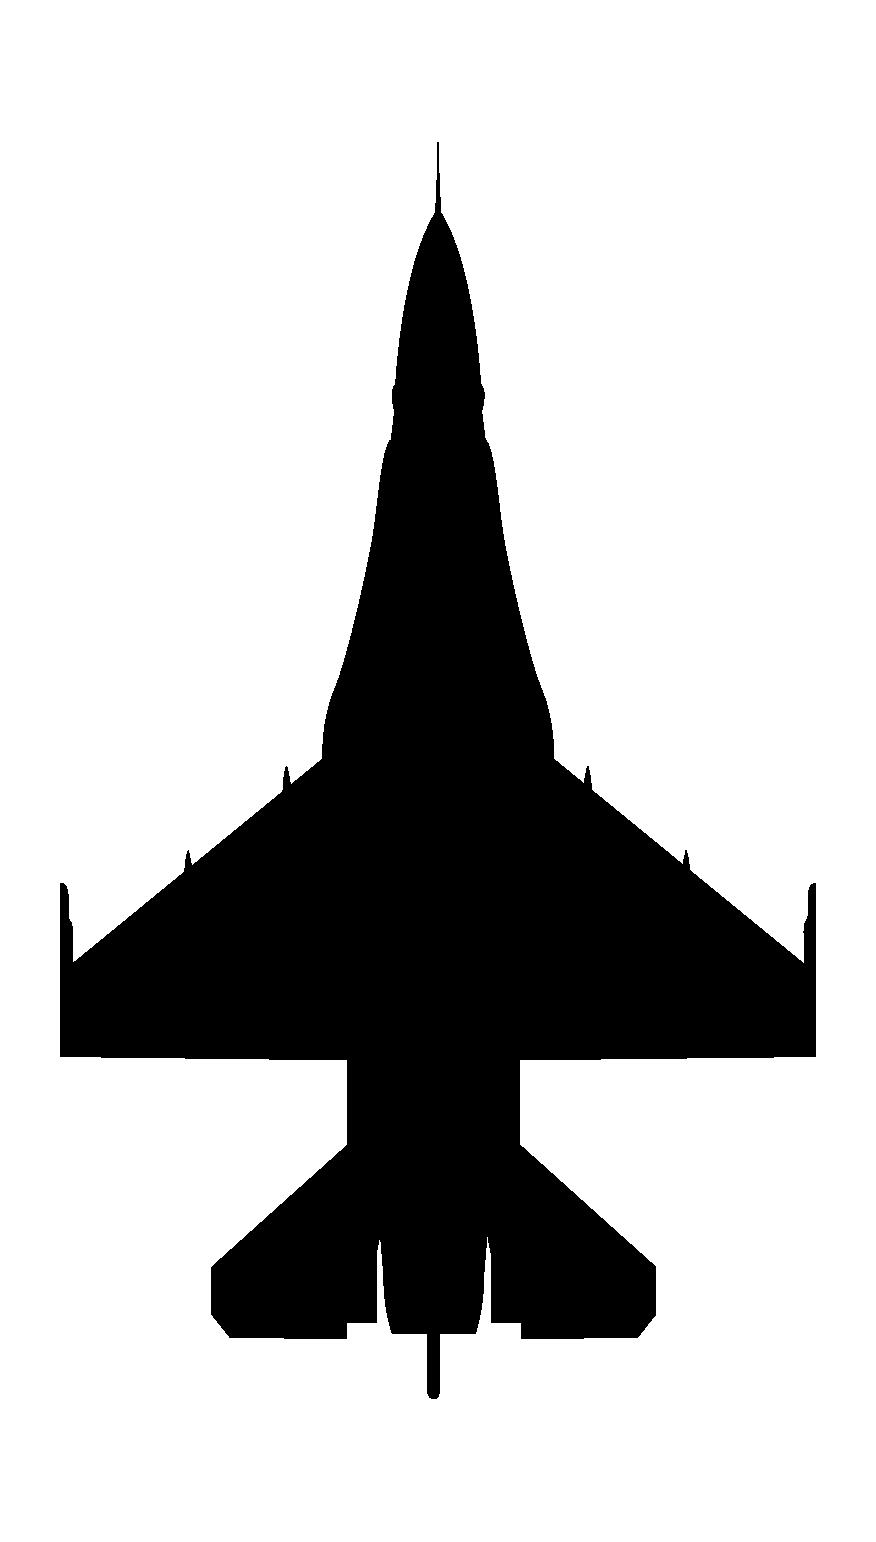
\includegraphics[
                width=7.5mm,
            ]{diagrams/aircraft/silhouette_f16_top.pdf}
        };
        \node[below] (wing_hot_fig) at (wing_hot) {
            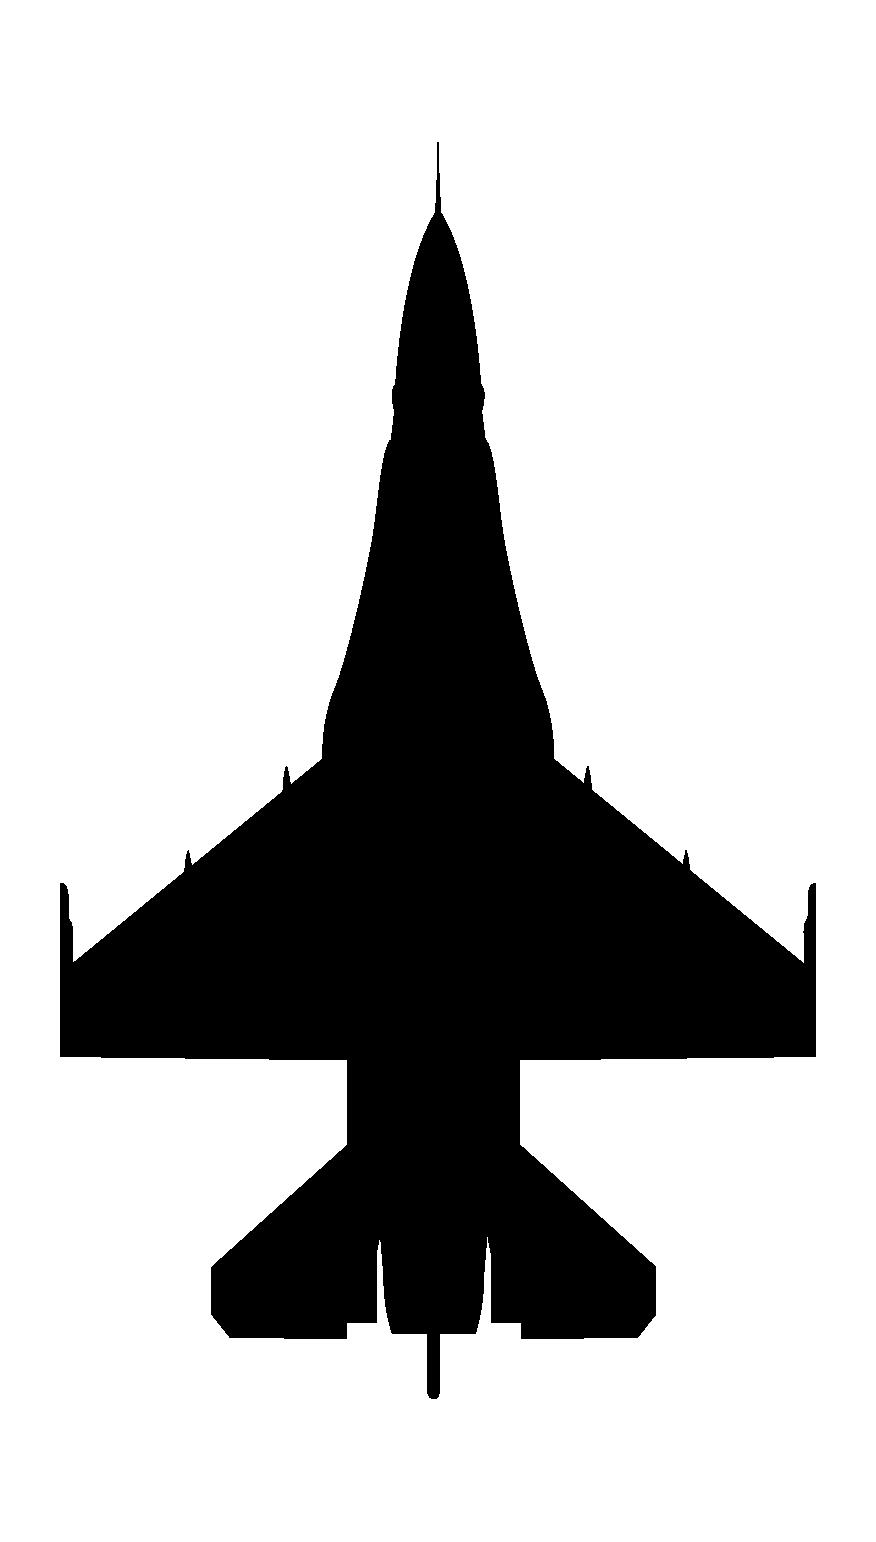
\includegraphics[
                width=7.5mm,
            ]{diagrams/aircraft/silhouette_f16_top.pdf}
        };
        \node[below, rotate=180] (lead_cold_fig) at (lead_cold) {
            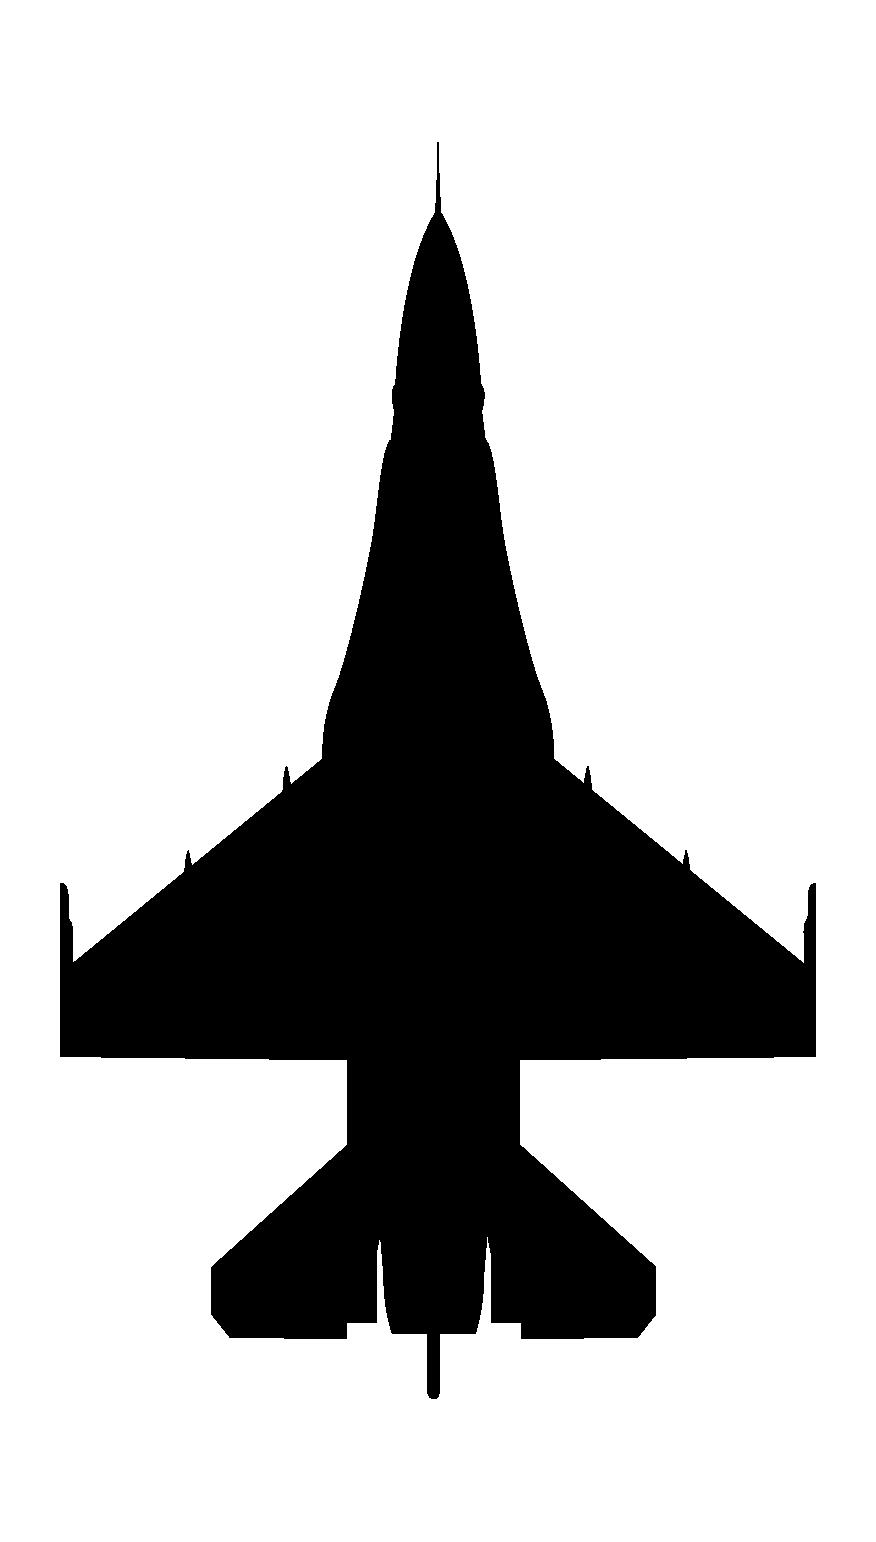
\includegraphics[
                width=7.5mm,
            ]{diagrams/aircraft/silhouette_f16_top.pdf}
        };
        \node[below, rotate=180] (wing_cold_fig) at (wing_cold) {
            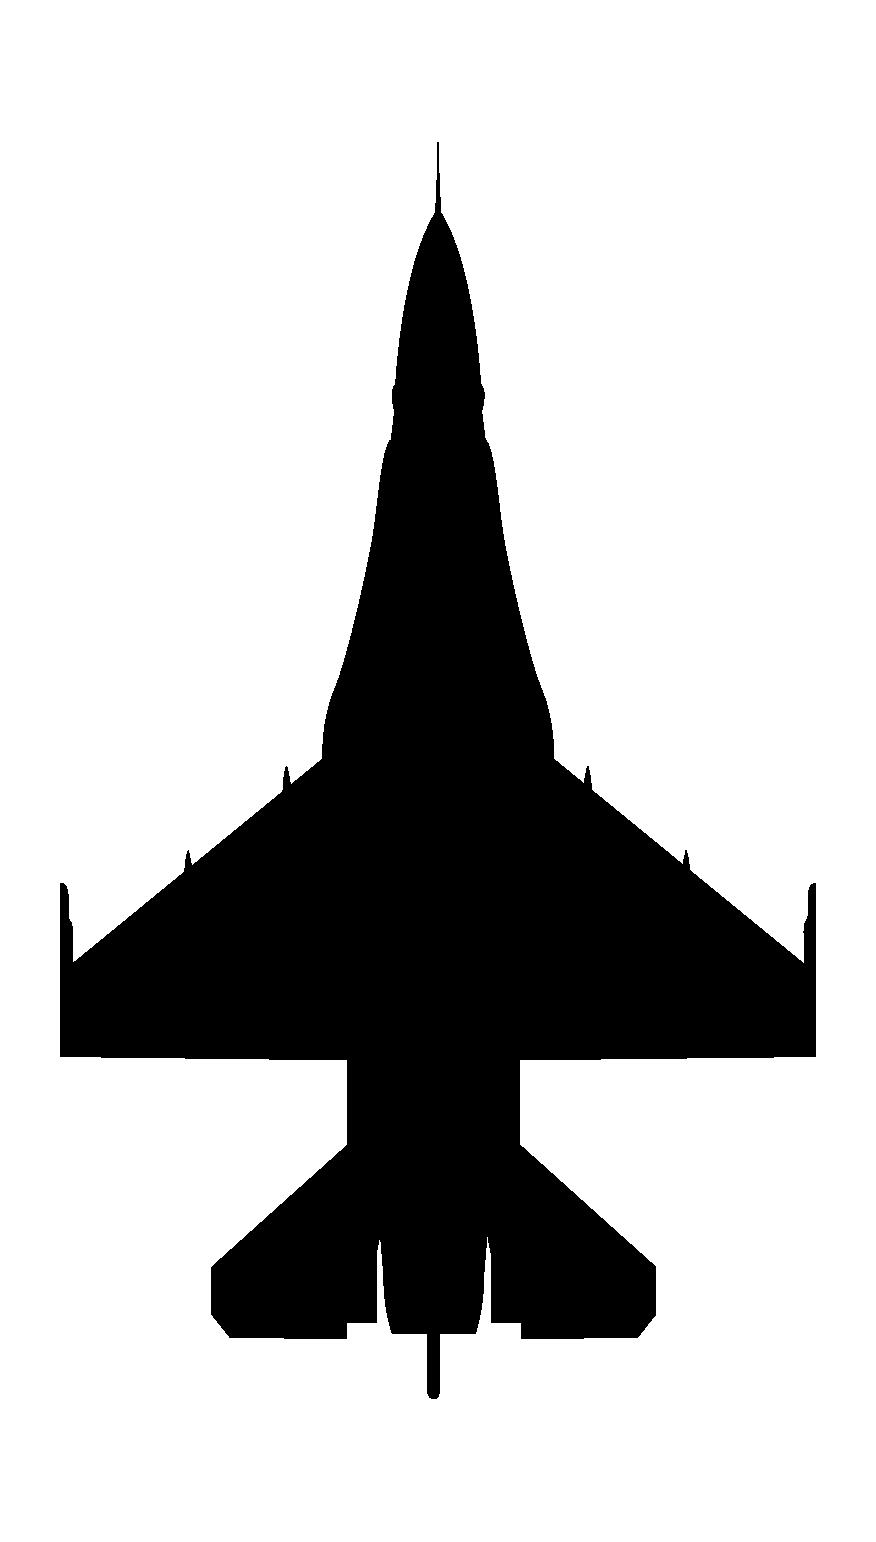
\includegraphics[
                width=7.5mm,
            ]{diagrams/aircraft/silhouette_f16_top.pdf}
        };
        
        \foreach \n in {lead, wing} {
        \draw[->] 
                (\n_hot) 
            -- ++(0,5)
            arc (180:0:10) 
                -- (\n_cold_fig.south);
        \draw[->] 
                (\n_cold) 
            -- ++(0,-5)
            arc (0:-180:10) 
                -- (\n_hot_fig.south);
        }

        % bandit
        \node[] (bandit_fig) at (bandit) {
            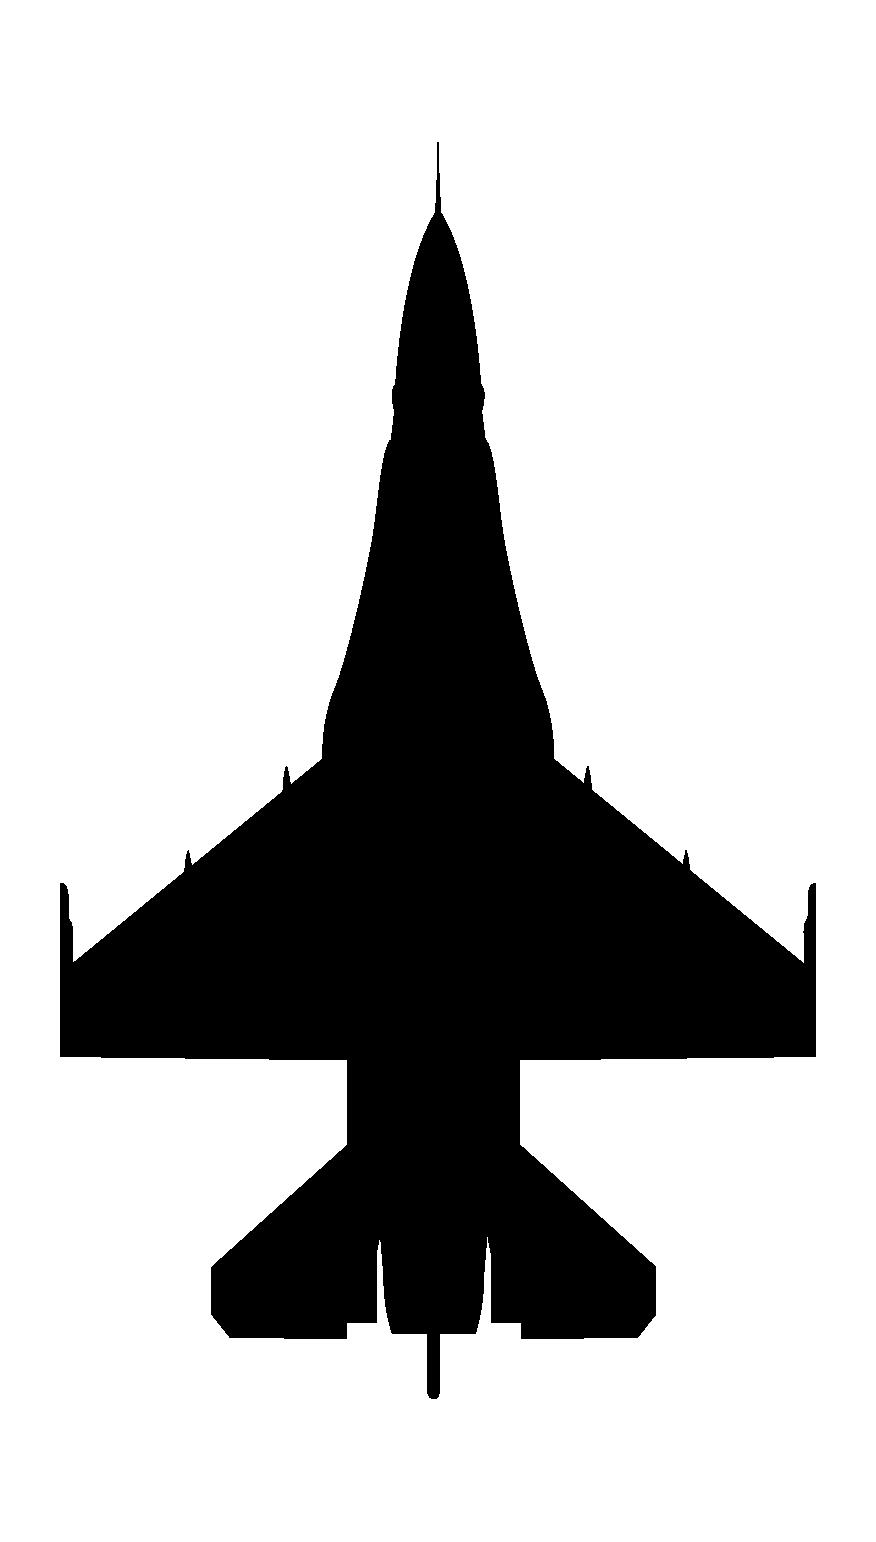
\includegraphics[
                    angle=180,
                    width=7.5mm,
            ]{diagrams/aircraft/silhouette_f16_top.pdf}
        };
        \node[] at (bandit_wing) {
            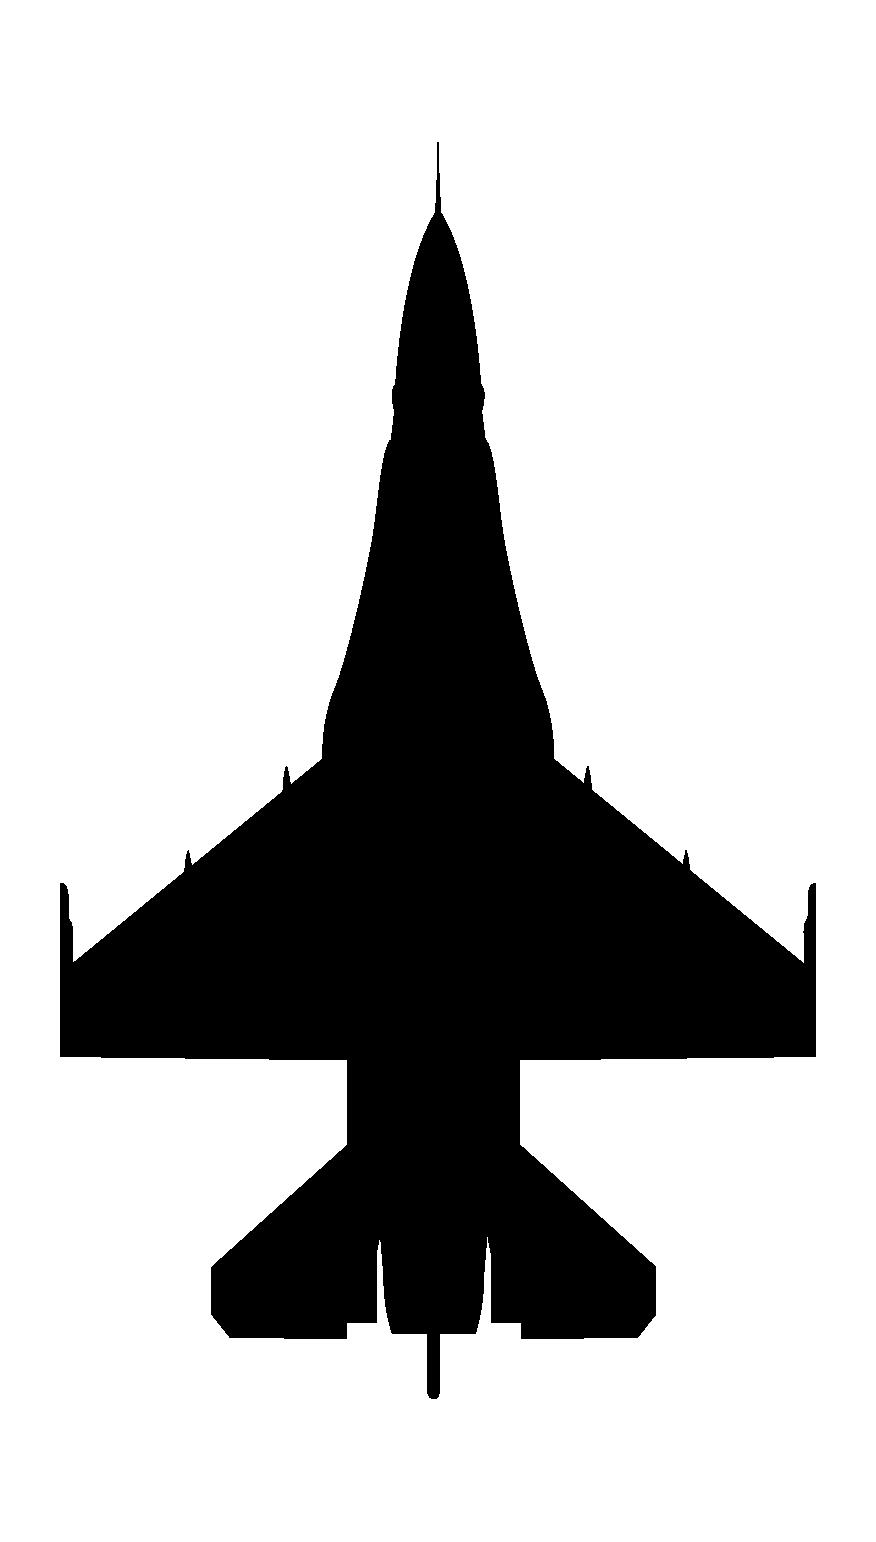
\includegraphics[
                    angle=180,
                    width=7.5mm,
            ]{diagrams/aircraft/silhouette_f16_top.pdf}
        };

        % labels
        \node[font=\small, align=right, left] at (wing_hot_fig.west) {Hot \\ Element};
        \node[font=\small, align=left, right] at (lead_cold_fig.west) {Cold \\ Element};
        \node[font=\small, right] at (bandit_fig.east) {Bandits};

    \end{tikzpicture}
    \caption{Four-ship grinder tactics}%
    \label{fig:ttp_aa:4ship:offensive:grinder}
\end{figure}

\subsection{DEFENSIVE TACTICS}